\documentclass[11pt]{article}
\usepackage{mathtools}
\usepackage{mdframed}
\usepackage{fullpage}
\usepackage{amsfonts}
\usepackage{tikz}
\usepackage{fancyhdr}
\usepackage{lastpage}
\usepackage{enumitem}
\usepackage{graphicx}

%edit this for each class
\newcommand\name{John Collin Vincent}
\newcommand\classname{Com S 486}
\newcommand\assignment{homework 4}


\newcounter{excounter}
\setcounter{excounter}{1}
\newcommand\ques[2]{\vskip 1em  \noindent\textbf{\arabic{excounter}\addtocounter{excounter}{1}.} \emph{#1} \noindent#2}
\newenvironment{question}{\ques{}\begin{quote}}{\end{quote}}
\newenvironment{subquestion}[1]{#1) \begin{quote}}{\end{quote}}

\pagestyle{fancy}
\rfoot{\name, page \thepage/\pageref{LastPage}}
\cfoot{}
\rhead{}
\lhead{}
\renewcommand{\headrulewidth}{0pt}
\renewcommand{\footrulewidth}{0pt}
\DeclarePairedDelimiter\ceil{\lceil}{\rceil}
\DeclarePairedDelimiter\floor{\lfloor}{\rfloor}


\begin{document}


    {\bf \classname \hspace{1cm} \assignment\hfill \name}
    \vskip 2em


    \begin{question}
        \begin{tabular}{ l r c c c c c c }
                 &      &    &  & D(v) & D(x)   & D(y)   & D(z)\\
            Step & N'   & D(w),p(w) & D(t),p(t) & p(v) & p(x)   & p(y)   & p(z)\\\hline
            0    & u    & 3,u       &(2,u )     & 3,u  &$\infty$&$\infty$&$\infty$\\\hline
            1    & ut   & (3,u)     &           & 3,u  &$\infty$& 9,y    &$\infty$\\\hline
            2    & utw  &           &           & (3,u)& 9,x    & 9,y    &$\infty$\\\hline
            3    & utwv &           &           &      & (6,x)  & 9,y    &$\infty$\\\hline
            4    & utwvx&           &           &      &        & (9,y)  & 14,x   \\\hline
            5    &utwvxy&           &           &      &        &        & (14,x) \\\hline
            6    &utwvxyz&          &           &      &        &        &        \\\hline
        \end{tabular}
    \end{question}

    \begin{question}
        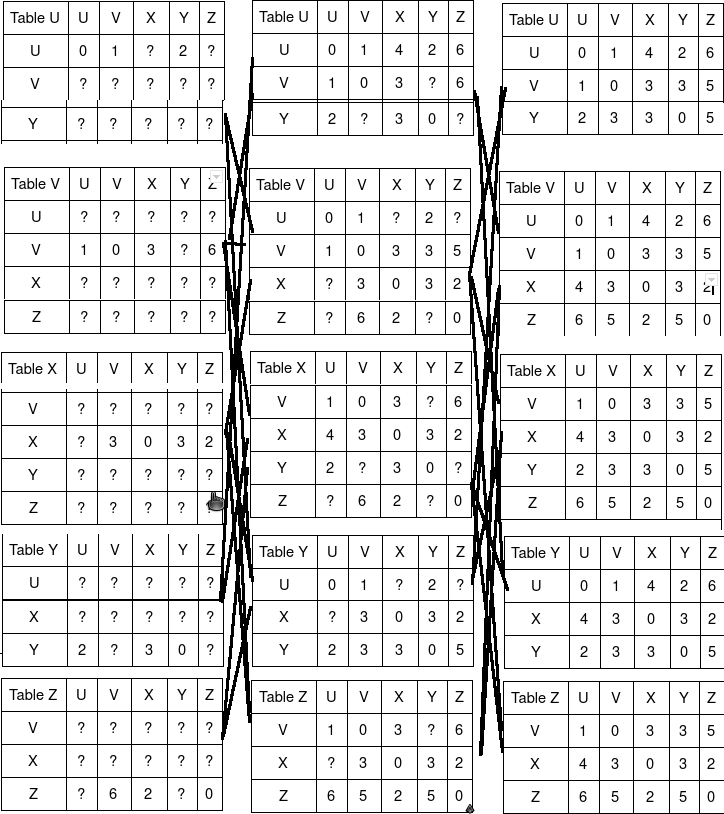
\includegraphics[scale=1.5]{coms486/hw4/usable.png} 
    \end{question}

    \begin{question}
        \begin{enumerate}[label=(\alph*)]
            \item OSPF from 4a to 4c, then eBGP from 4c to 3c, then iBGP from 3c to 3b and 3a
            \item 1a
            \item 1a
        \end{enumerate}
    \end{question}

    \begin{question}
        \begin{tabular}{ | l | l | l | l | l |}
            \hline
            1 & 0 & 1 & 1 & \color{blue}{1}\\ \hline
            0 & 1 & 0 & 0 & \color{blue}{1}\\ \hline
            1 & 0 & 1 & 1 & \color{blue}{1}\\ \hline
            1 & 1 & 1 & 1 & \color{blue}{0}\\ \hline
            \color{blue}{1} & \color{blue}{0} & \color{blue}{1} & \color{blue}{1} & \color{blue}{1} \\ \hline
        \end{tabular}

        parity bits: 111010111
    \end{question}

    \begin{question}
        a) $R = 1001$\\
        b) $R = 0101$\\
    \end{question}

    \begin{question}
        \begin{enumerate}[label=(\alph*)]
            \item A to B success = $P_A(1 - P_B)$\\
                  B to A sends success =  $P_B(1 - P_A)$\\
                  A or B is a success: $P_A(1 - P_B) + P_B(1 - P_A)$\\
                  A collides with B: $P_A * P_B$\\
                  A and B don't send: $(1-P_A) * (1-P_B) $a
            \item A's average throughput is $P_A(1-P_B)*\text{number of slots}$\\
                  B's average throughput is $P_B(1-P_A)*\text{number of slots}$
        \end{enumerate}
        
    \end{question}

\end{document}
